%% LaTeX-Beamer template for KIT design
%% by Erik Burger, Christian Hammer
%% title picture by Klaus Krogmann
%%
%% version 2.1
%%
%% mostly compatible to KIT corporate design v2.0
%% http://intranet.kit.edu/gestaltungsrichtlinien.php
%%
%% Problems, bugs and comments to
%% burger@kit.edu

\documentclass[18pt]{beamer}

%% SLIDE FORMAT

% use 'beamerthemekit' for standard 4:3 ratio
% for widescreen slides (16:9), use 'beamerthemekitwide'

\usepackage{./templates/beamerthemekit}
% \usepackage{templates/beamerthemekitwide}


\titleimage{kde-and-trajectories}



\title{Kernel Density Estimates and Mean Shift Clustering}
% \subtitle{Sommersemester 2018}
\author{Jonas Spinner}
\date{February 4, 2019}

\institute{Analytics and Statistics at the Institute of Operations Research}

% Bibliography

\usepackage{natbib}

%\usepackage[citestyle=authoryear,bibstyle=numeric,hyperref,backend=biber]{biblatex}
%\addbibresource{../latex/KDEaMSC.bib}
%\bibhang1em


%\usepackage{tikz}

%\usepackage{algorithm}
%\usepackage{algorithmic}

\usepackage{algpseudocode}
\usepackage{algorithm}
% keine "End"-Statements in Algorithmen
\algtext*{EndWhile}
\algtext*{EndIf}
\algtext*{EndFor}
\algtext*{EndProcedure}


\usepackage[utf8]{inputenc}
\usepackage[english]{babel}
\usepackage[T1]{fontenc}
\usepackage{amsmath,amsmath,lmodern}
\usepackage{bm}
\usepackage{bbm}

\usepackage{graphicx}
\usepackage{subfig}

\usepackage[font=scriptsize]{caption}



\newcommand{\norm}[1]{\left\lVert#1\right\rVert}



\begin{document}

% change the following line to "ngerman" for German style date and logos
% \selectlanguage{ngerman}

%title page
\begin{frame}
\titlepage
\end{frame}

%table of contents
\begin{frame}{Outline}
	\tableofcontents
\end{frame}


\section{Introduction}


\section{Kernel Density Estimates}

\begin{frame}{Density estimation}
	\begin{figure}
		\tiny
		\centering
		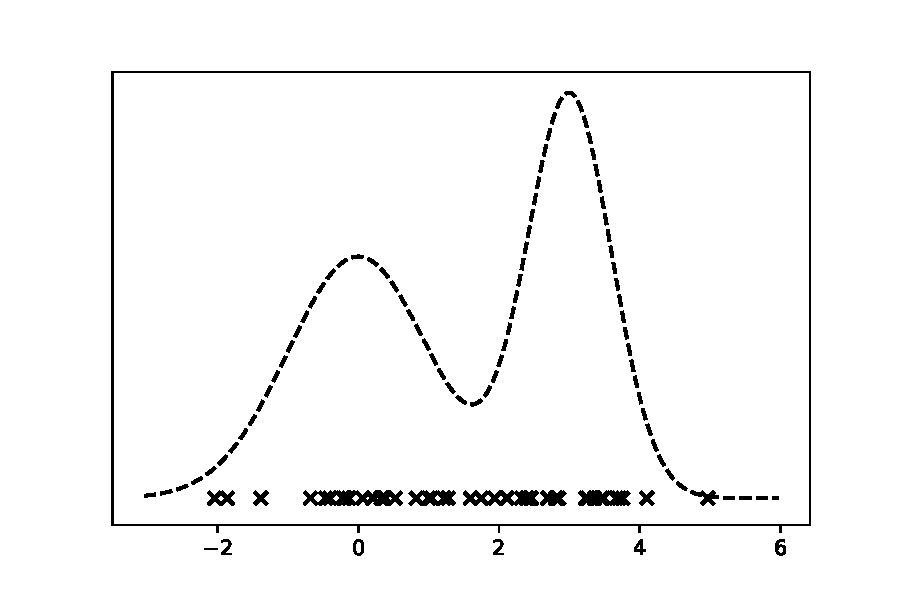
\includegraphics[height=0.5\textheight]{figures/samples-and-underlying-pdf}
		%\vspace*{-4mm}
		%\caption{Author's illustration.}
	\end{figure}
	\vspace*{-4mm}
	\begin{itemize}
		\item \textbf{Task}: Given samples $\bm{x}_1, ..., \bm{x}_n \in \mathbb{R}^d$, estimate the underlying density.
		%\item \textbf{Assumptions}: $\bm{x}_i$ are independent and identically distributed with probability density distribution $f(\bm{x})$.
	\end{itemize}
\end{frame}


\subsection{Definition}

\begin{frame}{The kernel density estimate}
	The \textbf{kernel density estimate} is defined as
	\begin{align*}
		\hat{f}(\bm{x}) = \frac{1}{n h^d} \sum_{i=1}^{n} K\left(\frac{\bm{x} - \bm{x}_i}{h} \right)
	\end{align*}
	
	\begin{itemize}
		\item $K$ is a \textit{kernel function}.
		\item $h$ is a \textit{bandwidth parameter}.
	\end{itemize}
	\begin{itemize}
		\item When $\int_{\mathbb{R}^d} K(\bm{x}) d\bm{x} = 1$ and $K(\bm{x}) \geq 0$ for all $\bm{x}$ then $\hat{f}(\bm{x})$ is a valid probability density function.
	\end{itemize}
\end{frame}


\begin{frame}{The kernel density estimate}
	\begin{align*}
		\hat{f}(\bm{x}) = \frac{1}{n h^d} \sum_{i=1}^{n} K\left(\frac{\bm{x} - \bm{x}_i}{h} \right)
	\end{align*}
	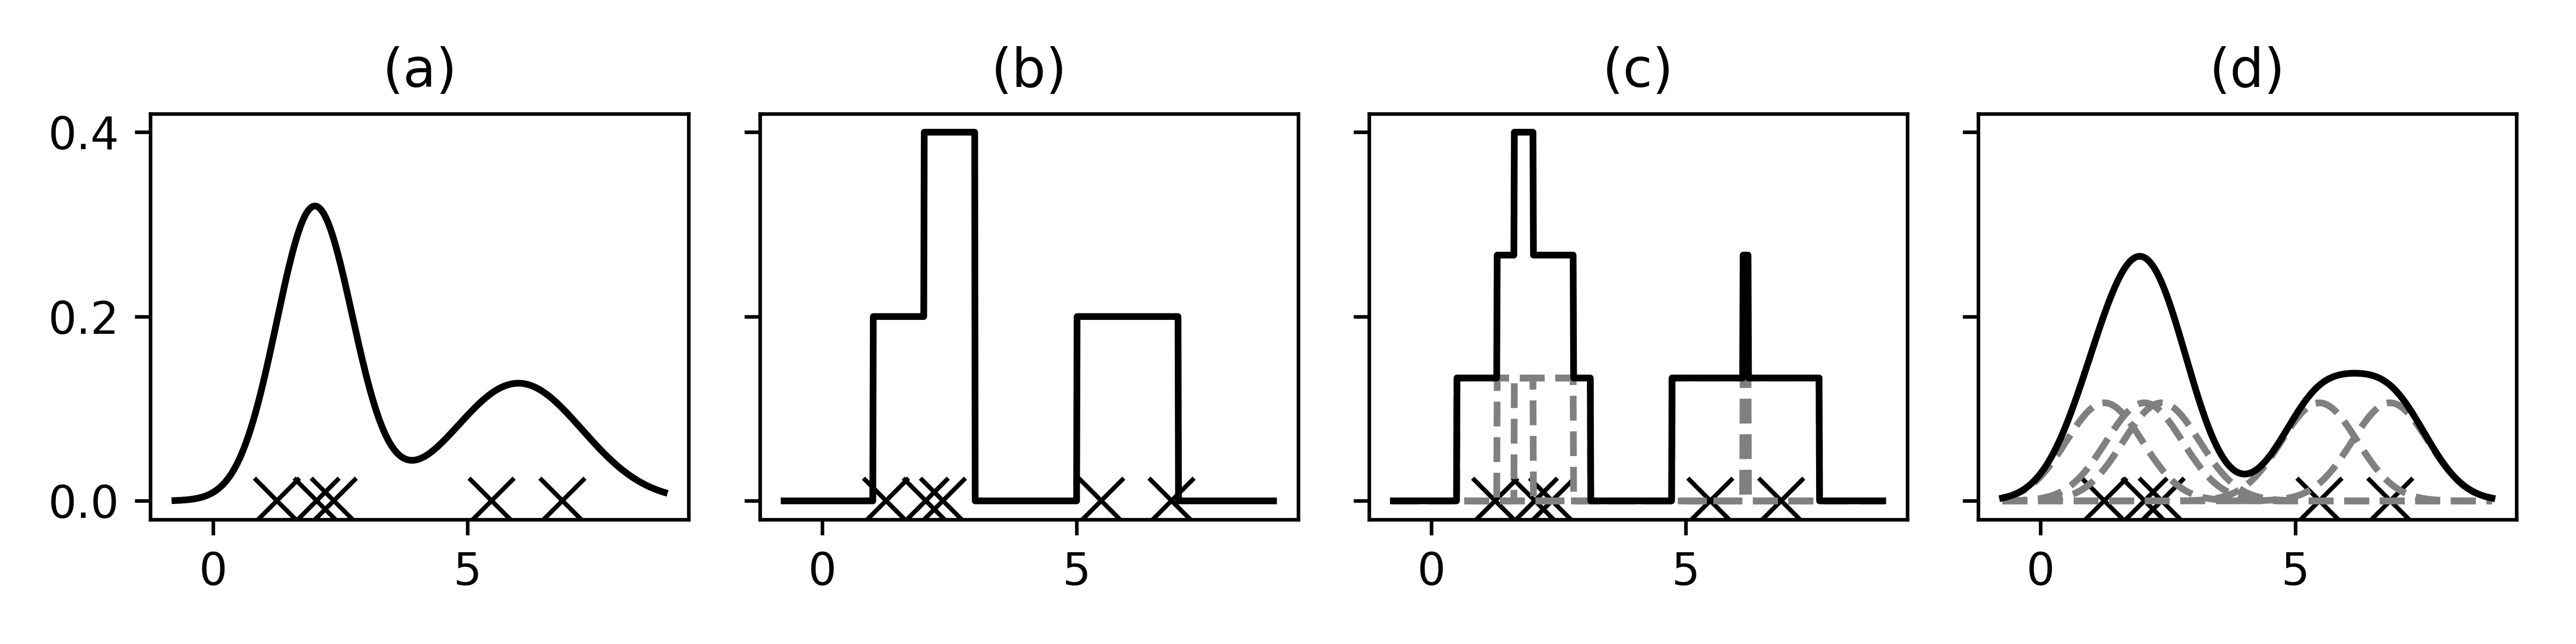
\includegraphics[width=\textwidth]{figures/kde-kernel-density-estimates}
	\vspace*{-5mm}
	\tiny
	\begin{itemize}
		\item[(a)] Underlying density.
		\item[(b)] Histogram.
		\item[(c)] KDE with uniform kernel.
		\item[(d)] KDE with gaussian kernel.
	\end{itemize}
\end{frame}


\subsection{Kernel functions}

\begin{frame}{Popular kernel functions}
	\textbf{Radially symmetric kernel functions} are kernel functions which can be represented as
	\begin{align*}
		K(\bm{x}) = c_{k,d}\ k\left(\norm{\bm{x}}^2\right)
	\end{align*}
	
	\begin{itemize}
		\item $k(u) : [0, \infty) \rightarrow [0, \infty)$ is called the \textbf{profile} of $K$.
		\item For example the gaussian kernel has the profile $k(u) = \exp(-\frac{1}{2}u)$.
		\item Nearly all popular kernel belong to this class of kernels.
	\end{itemize}
\end{frame}


\begin{frame}{Popular kernel functions}
	\centering
	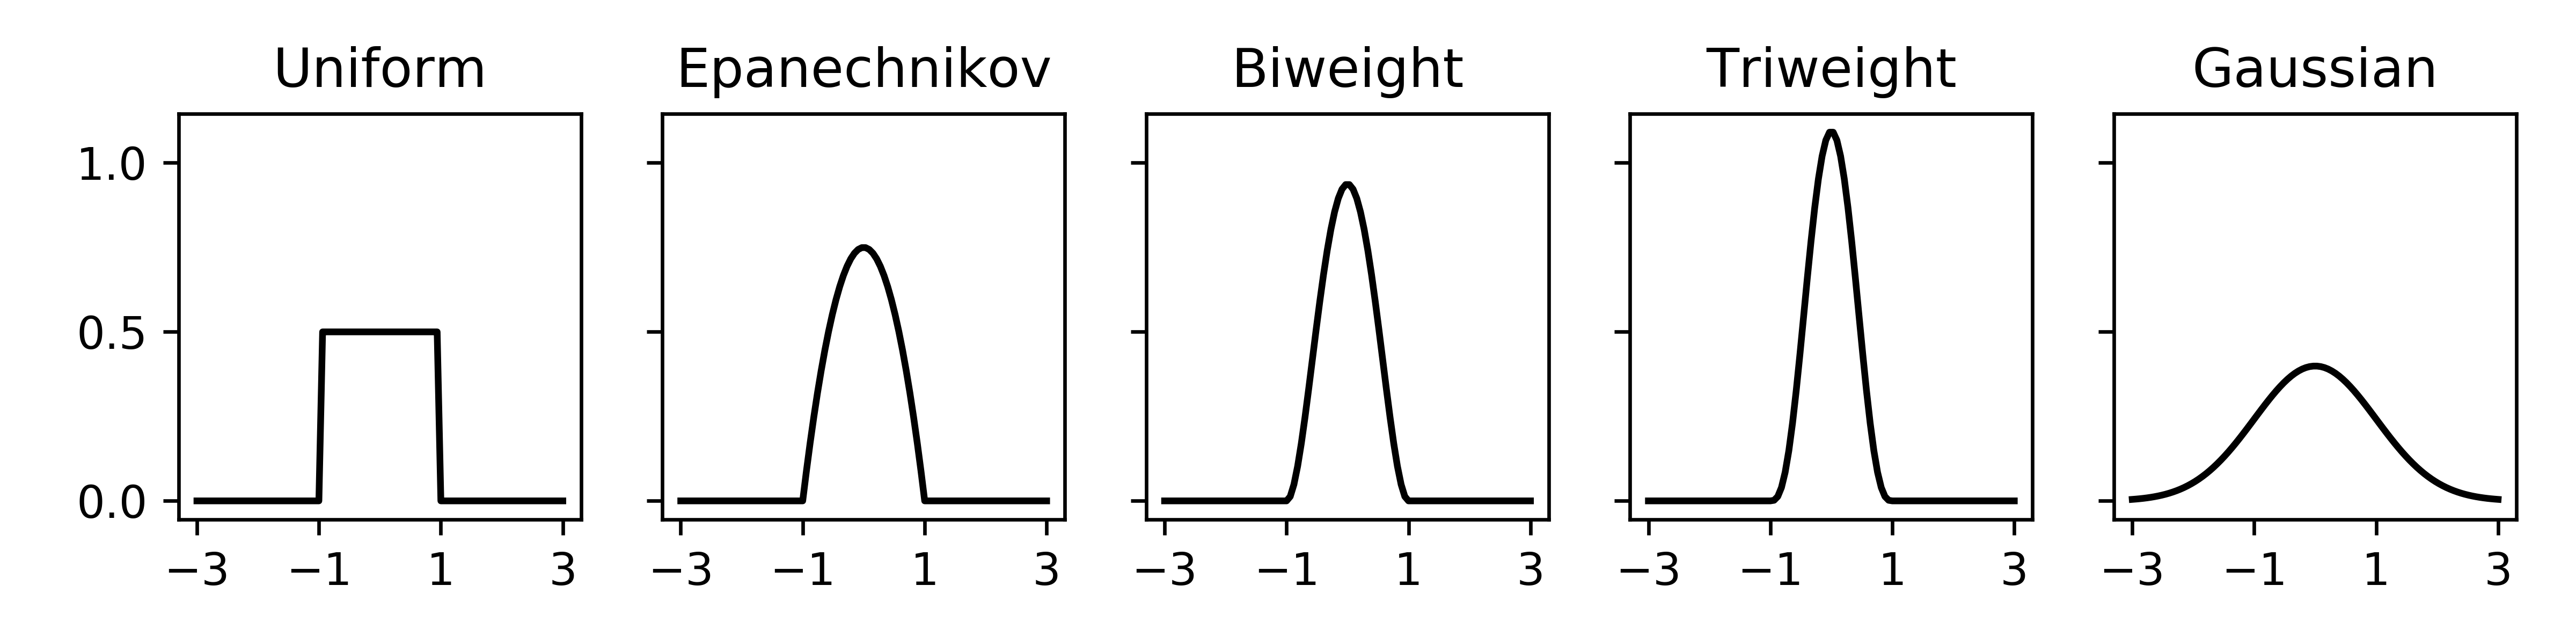
\includegraphics[width=0.9\textwidth]{figures/kde-popular-kernels}
	\begin{table}
		\begin{center}
			\tiny
			\begin{tabular}{r|r|r|r|l}
				\textbf{Name} & \textbf{Profile support} & $k(u)$ & $-k'(u)$ & $K(\bm{x})$ \\ \hline\hline
				Uniform & $u \in [0, 1]$ & $1$ & $0$ & $\text{vol}\left(S_d\right)^{-1}$ \\
				Epanechnikov & $u \in [0, 1]$ & $1 - u$ & $1$ & $\frac{1}{2} \text{vol}(S_d)^{-1} (d+2) \left(1 - \norm{\bm{x}}^2\right)$\\
				Biweight & $u \in [0, 1]$ & $(1 - u)^2$ & $2 (1 - u)$ & $\propto \left(1 - \norm{\bm{x}}^2\right)^2$ \\
				Triweight & $u \in [0, 1]$ & $(1 - u)^3$ & $3 (1 - u)^2$ & $\propto \left(1 - \norm{\bm{x}}^2\right)^3$ \\
				Gaussian & $u \in [0, \infty)$ & $\exp\left(-\frac{1}{2}u\right)$ & $\frac{1}{2}\exp\left(-\frac{1}{2}u\right)$ & $(2\pi)^{-d/2} \exp\left(-\frac{1}{2}\norm{\bm{x}}^2\right)$
			\end{tabular}
		\end{center}
	\end{table}
\end{frame}


\subsection{Bandwidth}

\begin{frame}{Bandwidth}
	\begin{figure}
		\includegraphics<1>[width=\textwidth]{figures/kernel-density-estimation-gaussian-50}
		\includegraphics<2>[width=\textwidth]{figures/kernel-density-estimation-uniform-50}
		\includegraphics<3>[width=\textwidth]{figures/kernel-density-estimation-epanechnikov-50}
		\vspace*{-6mm}
		\caption{\only<1>{Gaussian kernel}\only<2>{Uniform kernel}\only<3>{Epanechnikov kernel}, $n = 50$.}
	\end{figure}
	\begin{itemize}
		\item The choice of bandwidth is a bias-variance tradeoff for the estimate $\hat{f}(\bm{x})$.
		\item A small bandwidth results in high variance, a large bandwidth introduces a bias.
	\end{itemize}
\end{frame}



\section{Mean Shift Clustering}


\begin{frame}{Mean shift clustering}
	\centering
	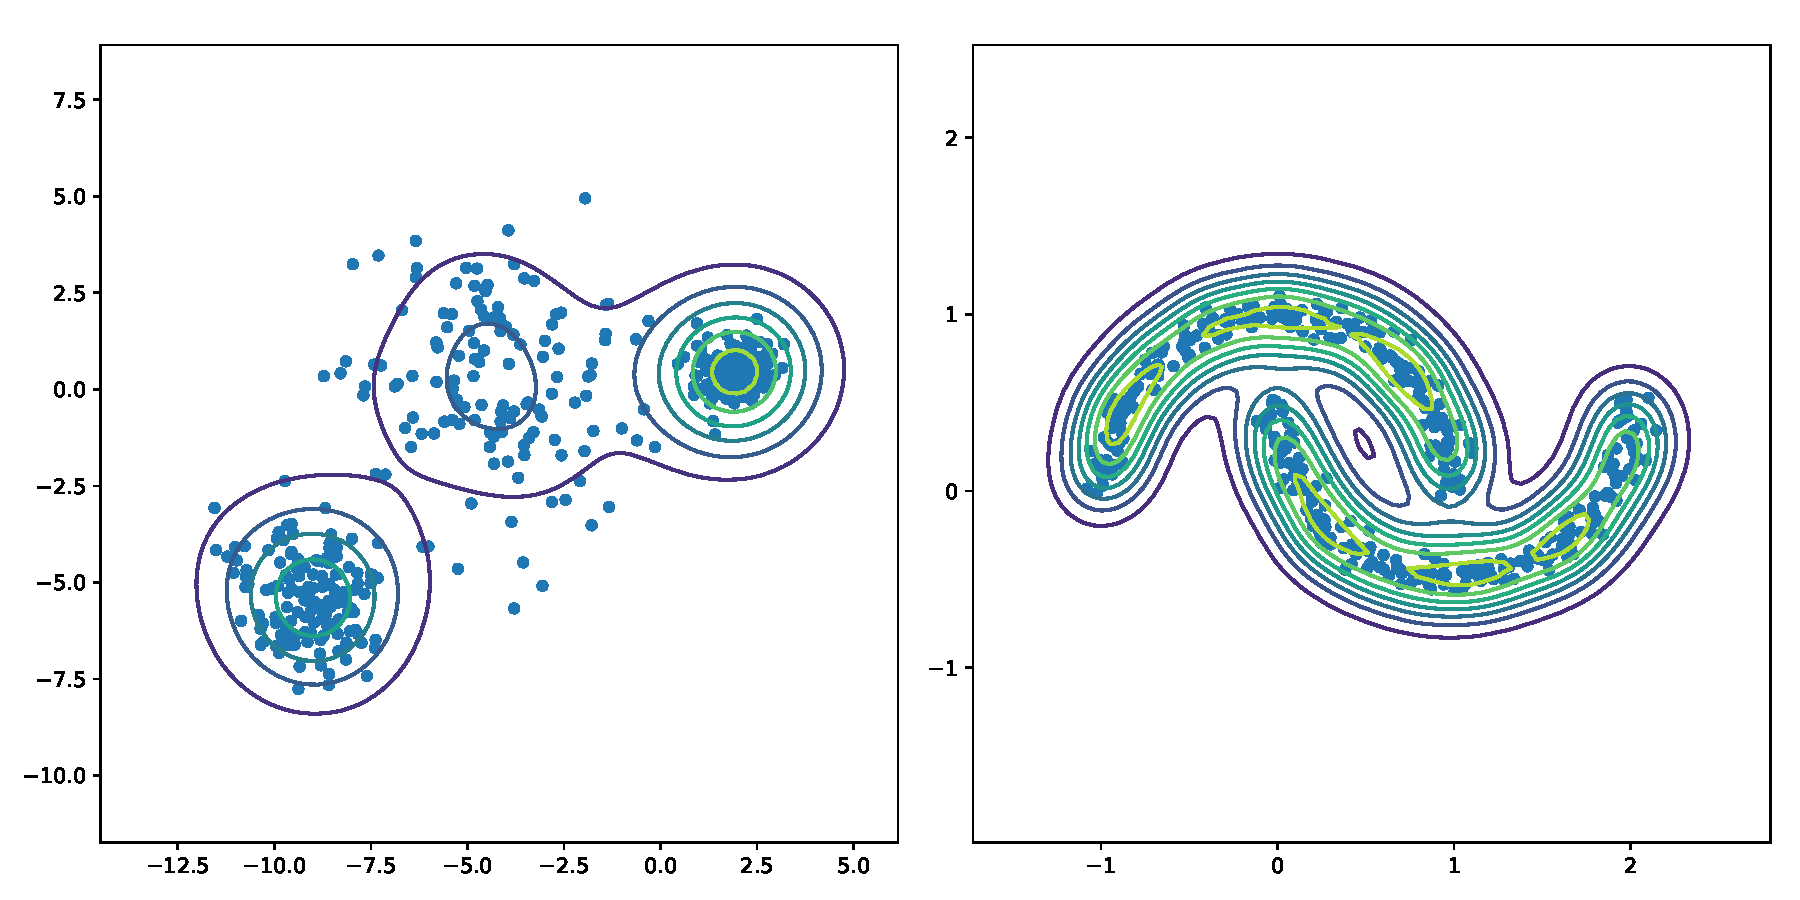
\includegraphics[height=0.5\textheight]{figures/mean-shift-introduction}
	\begin{itemize}
		\item Modes of the kernel density estimate can be used to identify clusters.
		\item Mode finding procedure results in a non-parametric clustering algorithm.
	\end{itemize}
\end{frame}


\subsection{Algorithm}
	
\begin{frame}{The idea}
	\centering
	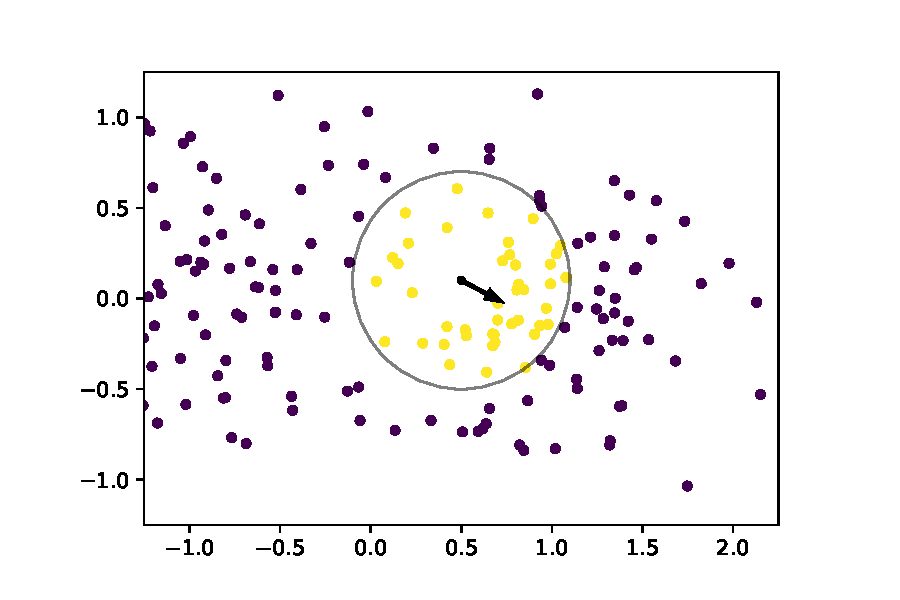
\includegraphics[width=0.7\textwidth]{figures/mean_shift_vector}
	\begin{itemize}
		\item Iteratively move point to ``high-density'' region.
		\item Direction is determined by local neighborhood.f
	\end{itemize}
\end{frame}



\begin{frame}{Locally weighted mean}
	The weighted mean is
	\begin{align*}
		\bm{\mu}^* = \frac{\sum_{i=1}^n \bm{x}_i w_i}{\sum_{i=1}^n w_i}
	\end{align*}
	\vspace*{10mm}
	
	The \textbf{locally weighted mean} has weights depending on the distance to a data point $\bm{x}$
	\begin{align*}
		\bm{\mu}^*(\bm{x}) = \frac{\sum_{i=1}^n \bm{x}_i\ g\left(\norm{\frac{\bm{x} - \bm{x}_i}{h}}^2 \right)}{\sum_{i=1}^n g\left(\norm{\frac{\bm{x} - \bm{x}_i}{h}}^2 \right)}
	\end{align*}
\end{frame}

\begin{frame}{Mean shift procedure}
	The \textbf{mean shift vector} is defined as
	\begin{align*}
		\bm{m}\left(\bm{x}\right) = \bm{\mu}^*(\bm{x}) - \bm{x}
	\end{align*}
	
	The \textbf{mean shift procedure} is
	\begin{align*}
		\bm{x}^{(t+1)} &= \bm{x}^{(t)} + \bm{m}\left(\bm{x}^{(t)}\right) & \text{for } i = 1, 2, ...
	\end{align*}
	
	\vspace*{5mm}
	\begin{itemize}
		\item When the process converges we assign $\bm{x}$ to the mode $\bm{x}^{(\infty)}$.
		\item Points at the same mode are considered to be in the same cluster.
	\end{itemize}
\end{frame}


\subsection{Convergence}

\begin{frame}{Convergence -- Gaussian kernel}
\includegraphics<1>[width=\textwidth]{figures/iterations-gaussian/step-1}
	\includegraphics<2>[width=\textwidth]{figures/iterations-gaussian/step-2}
	\includegraphics<3>[width=\textwidth]{figures/iterations-gaussian/step-3}
	\includegraphics<4>[width=\textwidth]{figures/iterations-gaussian/step-4}
	\includegraphics<5>[width=\textwidth]{figures/iterations-gaussian/step-5}
	\includegraphics<6>[width=\textwidth]{figures/iterations-gaussian/step-6}
	\includegraphics<7>[width=\textwidth]{figures/iterations-gaussian/step-7}
	\includegraphics<8>[width=\textwidth]{figures/iterations-gaussian/step-8}
	\includegraphics<9>[width=\textwidth]{figures/iterations-gaussian/step-9}
	\includegraphics<10>[width=\textwidth]{figures/iterations-gaussian/step-10}
	\includegraphics<11>[width=\textwidth]{figures/iterations-gaussian/step-11}
	\includegraphics<12>[width=\textwidth]{figures/iterations-gaussian/step-12}
	\includegraphics<13>[width=\textwidth]{figures/iterations-gaussian/step-13}
	\includegraphics<14>[width=\textwidth]{figures/iterations-gaussian/step-14}
	\includegraphics<15>[width=\textwidth]{figures/iterations-gaussian/step-15}
	\includegraphics<16>[width=\textwidth]{figures/iterations-gaussian/step-16}
	\includegraphics<17>[width=\textwidth]{figures/iterations-gaussian/step-17}
\end{frame}

\begin{frame}{Convergence -- Uniform kernel}
\includegraphics<1>[width=\textwidth]{figures/iterations-uniform/step-1}
	\includegraphics<2>[width=\textwidth]{figures/iterations-uniform/step-2}
	\includegraphics<3>[width=\textwidth]{figures/iterations-uniform/step-3}
	\includegraphics<4>[width=\textwidth]{figures/iterations-uniform/step-4}
	\includegraphics<5>[width=\textwidth]{figures/iterations-uniform/step-5}
	\includegraphics<6>[width=\textwidth]{figures/iterations-uniform/step-6}
	\includegraphics<7>[width=\textwidth]{figures/iterations-uniform/step-7}
	\includegraphics<8>[width=\textwidth]{figures/iterations-uniform/step-8}
	\includegraphics<9>[width=\textwidth]{figures/iterations-uniform/step-9}
	\includegraphics<10>[width=\textwidth]{figures/iterations-uniform/step-10}
	\includegraphics<11>[width=\textwidth]{figures/iterations-uniform/step-11}
	\includegraphics<12>[width=\textwidth]{figures/iterations-uniform/step-12}
	\includegraphics<13>[width=\textwidth]{figures/iterations-uniform/step-13}
\end{frame}


\subsection{Connection to KDE}

\begin{frame}{Connecting the mean shift vector and kernel density estimation}
	\begin{itemize}
		\item \textbf{Result}: the mean shift vector $\bm{m}(\bm{x})$ points into the gradient direction of a kernel density estimate. 
	\end{itemize}
	\begin{align*}
		\bm{m}(\bm{x}) = \bm{\mu}^*(\bm{x}) - \bm{x} = \frac{h^2c_{g,d}}{2c_{k,d}} \frac{\nabla \hat{f}_{h,K}(\bm{x})}{\hat{f}_{h,G}(\bm{x})}
	\end{align*}
\end{frame}

\begin{frame}{Connecting the mean shift vector and kernel density estimation}
	\begin{align*}
		\nabla \hat{f}_{h,K}(\bm{x}) &= \nabla \frac{c_{k,d}}{nh^d} \sum_{i=1}^n k\left(\norm{\frac{\bm{x} - \bm{x}_i}{h}}^2 \right)\\
		&= \frac{2c_{k,d}}{nh^{d+2}} \sum_{i=1}^n (\bm{x} - \bm{x}_i)k'\left(\norm{\frac{\bm{x} - \bm{x}_i}{h}}^2 \right)\\
		&= \frac{2c_{k,d}}{nh^{d+2}} \left[\sum_{i=1}^n g\left(\norm{\frac{\bm{x} - \bm{x}_i}{h}}^2 \right)\right] \left[\frac{\sum_{i=1}^n \bm{x}_i g\left(\norm{\frac{\bm{x} - \bm{x}_i}{h}}^2 \right)}{\sum_{i=1}^n g\left(\norm{\frac{\bm{x} - \bm{x}_i}{h}}^2 \right)} - \bm{x}\right]\\
		&= \frac{2c_{k,d}}{h^2c_{g,d}} \hat{f}_{h,G}(\bm{x}) \bm{m}(\bm{x})
	\end{align*}
	
	With $g(u) = -k'(u)$ and $G(\bm{x}) = c_{g,d} g(\norm{\bm{x}}^2)$.
\end{frame}

\begin{frame}{Connecting the mean shift vector and kernel density estimation}
\centering
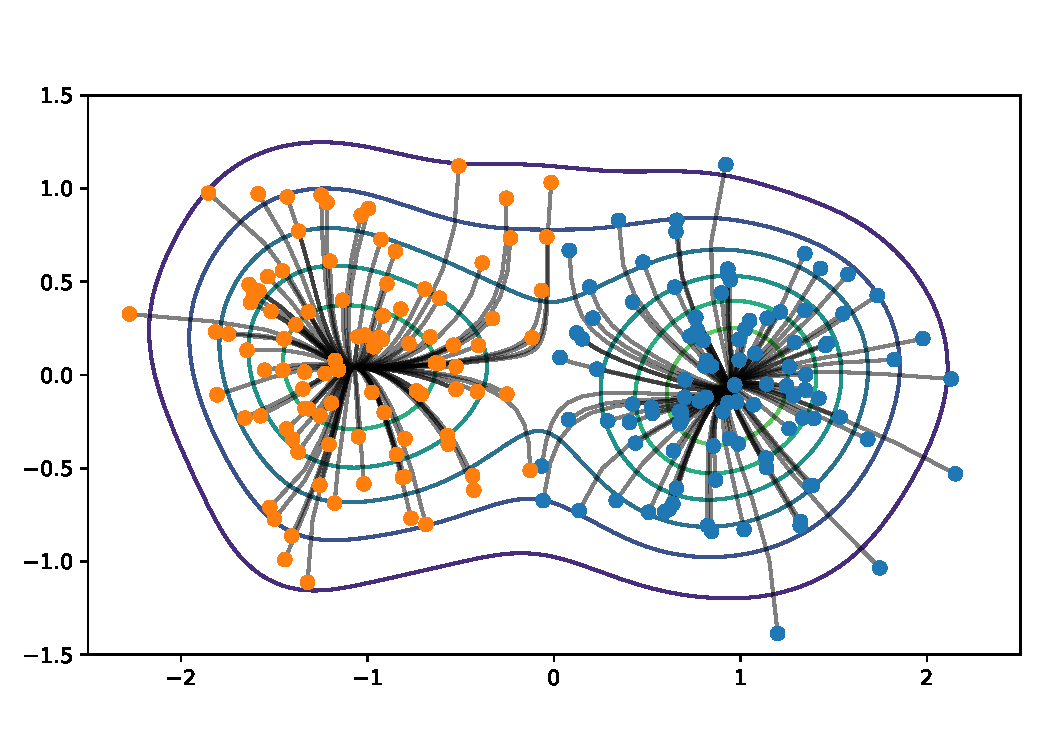
\includegraphics[height=0.4\textheight]{figures/contour}
	\begin{align*}
		\bm{m}(\bm{x}) = \frac{h^2c_{g,d}}{2c_{k,d}} \frac{\nabla \hat{f}_{h,K}(\bm{x})}{\hat{f}_{h,G}(\bm{x})}
	\end{align*}
	\begin{itemize}
		\item For the gaussian kernel $k(u) \propto -k'(u) = g(u)$ and therefore $K = G$.
	\end{itemize}
\end{frame}

\begin{frame}{Connecting the mean shift vector and kernel density estimation}
\begin{table}
	\begin{center}
		\begin{tabular}{r|r|r}
			\textbf{Name} & $k(u)$ & $-k'(u)$ \\ \hline\hline
			Uniform & $1$ & $0$ \\
			Epanechnikov & $1 - u$ & $1$ \\
			Biweight & $(1 - u)^2$ & $2 (1 - u)$ \\
			Triweight & $(1 - u)^3$ & $3 (1 - u)^2$  \\
			Gaussian & $\exp\left(-\frac{1}{2}u\right)$ & $\frac{1}{2}\exp\left(-\frac{1}{2}u\right)$
		\end{tabular}
	\end{center}
	\vspace*{10mm}
	\begin{itemize}
		\item A kernel $K$ for which $-k'(u) = g(u)$, is called a \textbf{shadow} of $G$.
		\item Calculating the mean shift vector $\bm{m}(\bm{x})$ with $G$ does calculate the gradient direction of the kernel density estimate with $K$ as kernel.
	\end{itemize}
\end{table}
\end{frame}



\subsection{Bandwidth effects}

\begin{frame}{Bandwidth effects}
	\begin{itemize}
		\item The choice of bandwidth influences the density estimation and therefore the clustering outcome
	\end{itemize}
	\begin{itemize}
		\item Small bandwidth $\Rightarrow$ many density peaks / clusters
		\item Large bandwidth $\Rightarrow$ few peaks / clusters
	\end{itemize}
\end{frame}
\begin{frame}{Small bandwidth}
\begin{figure}
	\tiny
	\begin{tabular}{c}
		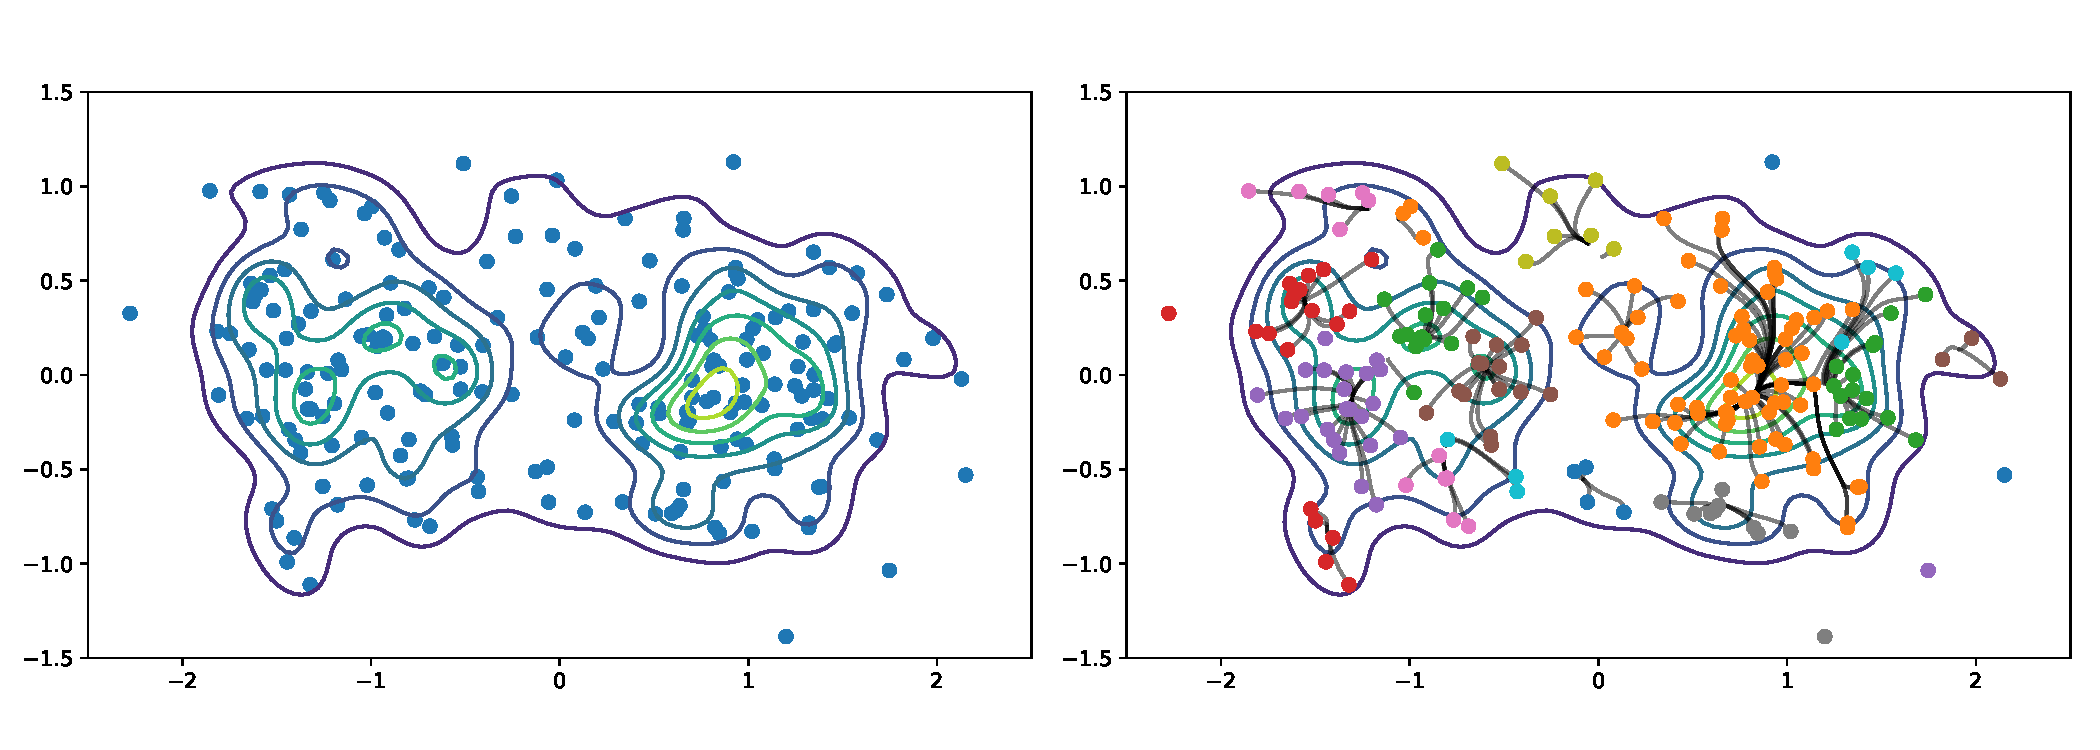
\includegraphics[height=0.4\textheight]{{{figures/contour/kde-and-trajectories-h=0.15-K=gaussian}}} \\[-2mm]
		$h=0.15$, gaussian kernel \\
		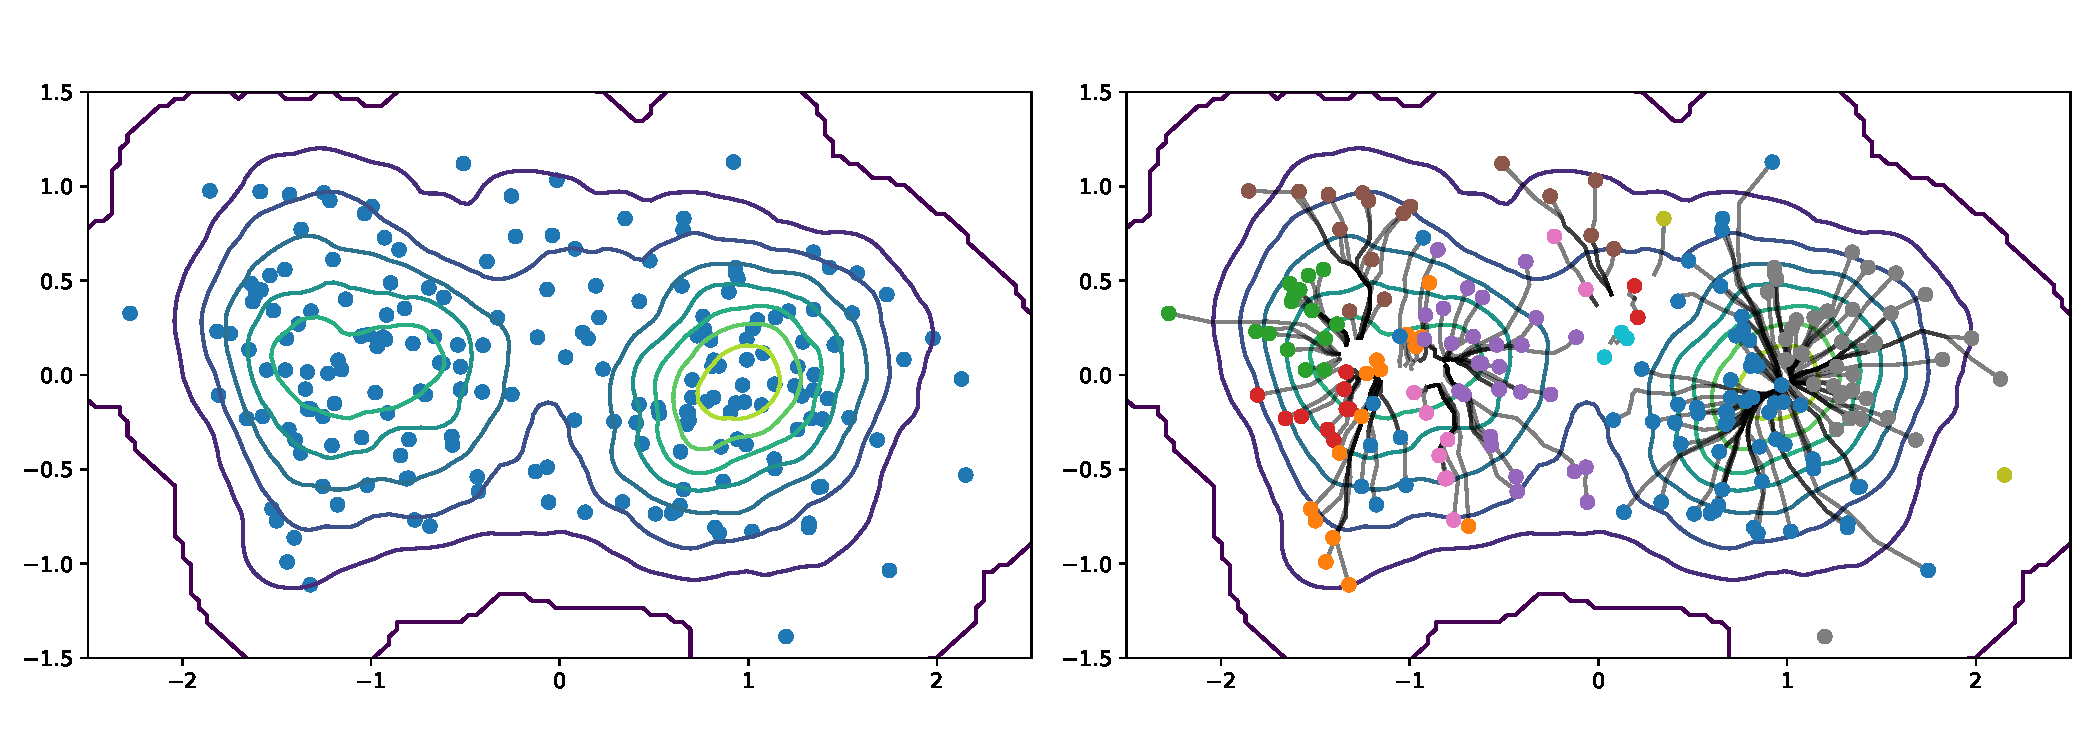
\includegraphics[height=0.4\textheight]{{{figures/contour/kde-and-trajectories-h=0.5-K=uniform}}} \\[-2mm]
		$h=0.5$, uniform kernel
	\end{tabular}
\end{figure}
\end{frame}

\begin{frame}{Medium bandwidth}
\begin{figure}	
	\tiny
	\begin{tabular}{c}
		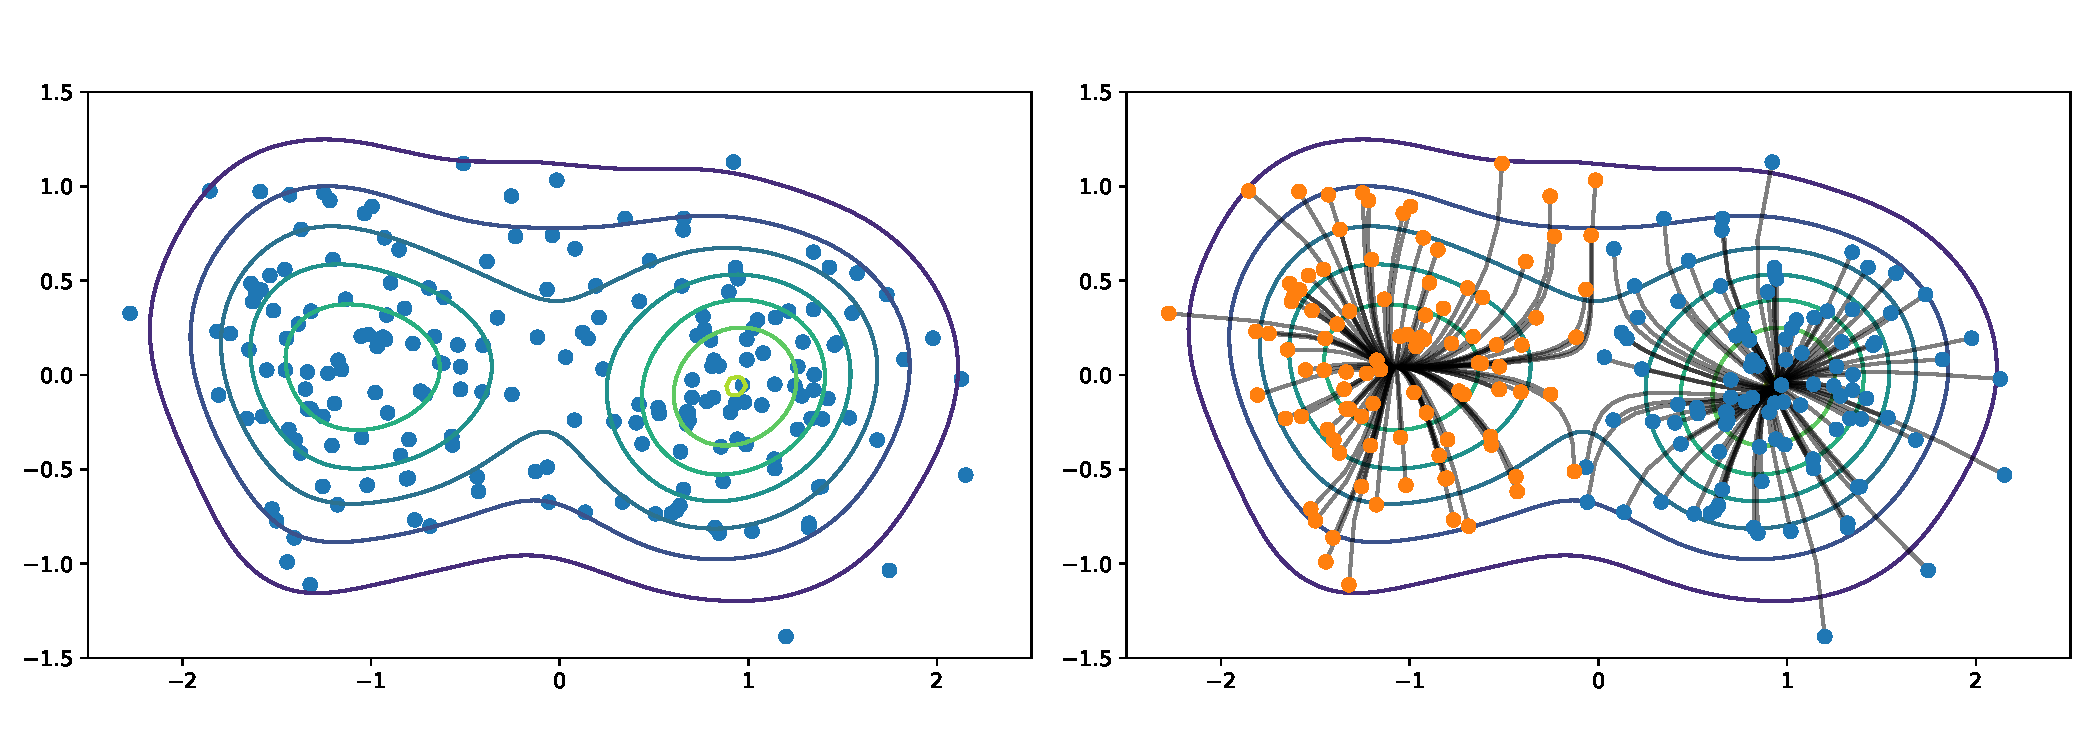
\includegraphics[height=0.4\textheight]{{{figures/contour/kde-and-trajectories-h=0.35-K=gaussian}}} \\[-2mm]
		$h=0.35$, gaussian kernel \\
		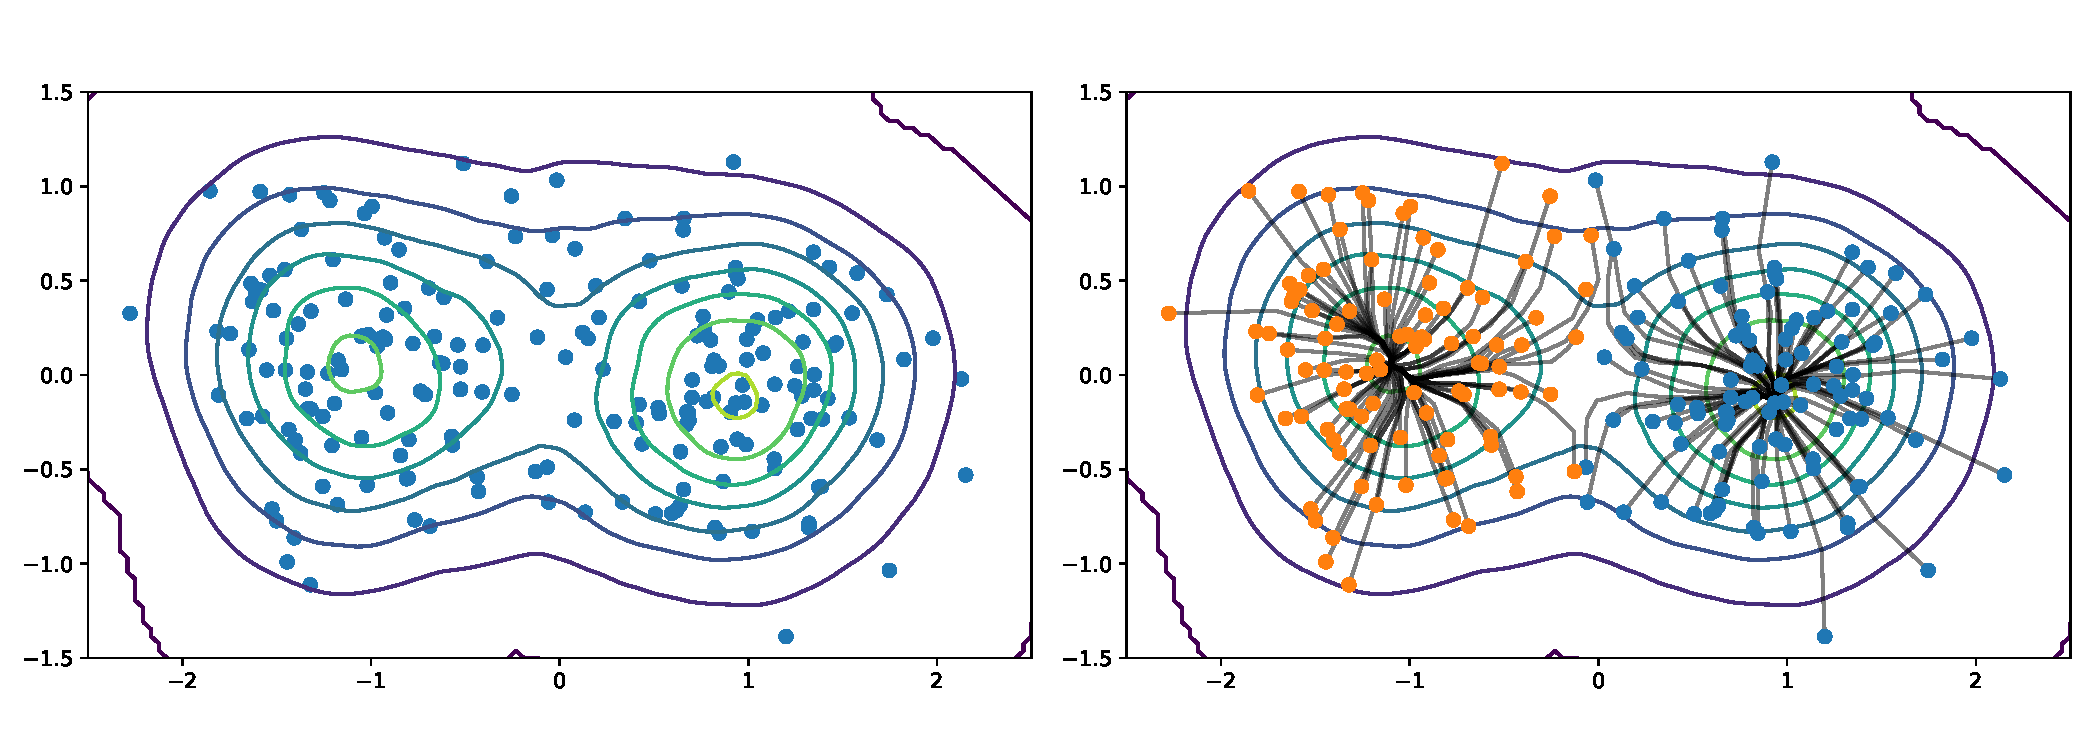
\includegraphics[height=0.4\textheight]{{{figures/contour/kde-and-trajectories-h=0.8-K=uniform}}} \\[-2mm]
		$h=0.8$, uniform kernel
	\end{tabular}
\end{figure}
\end{frame}

\begin{frame}{Large bandwidth}
\begin{figure}	
	\tiny
	\begin{tabular}{c}
		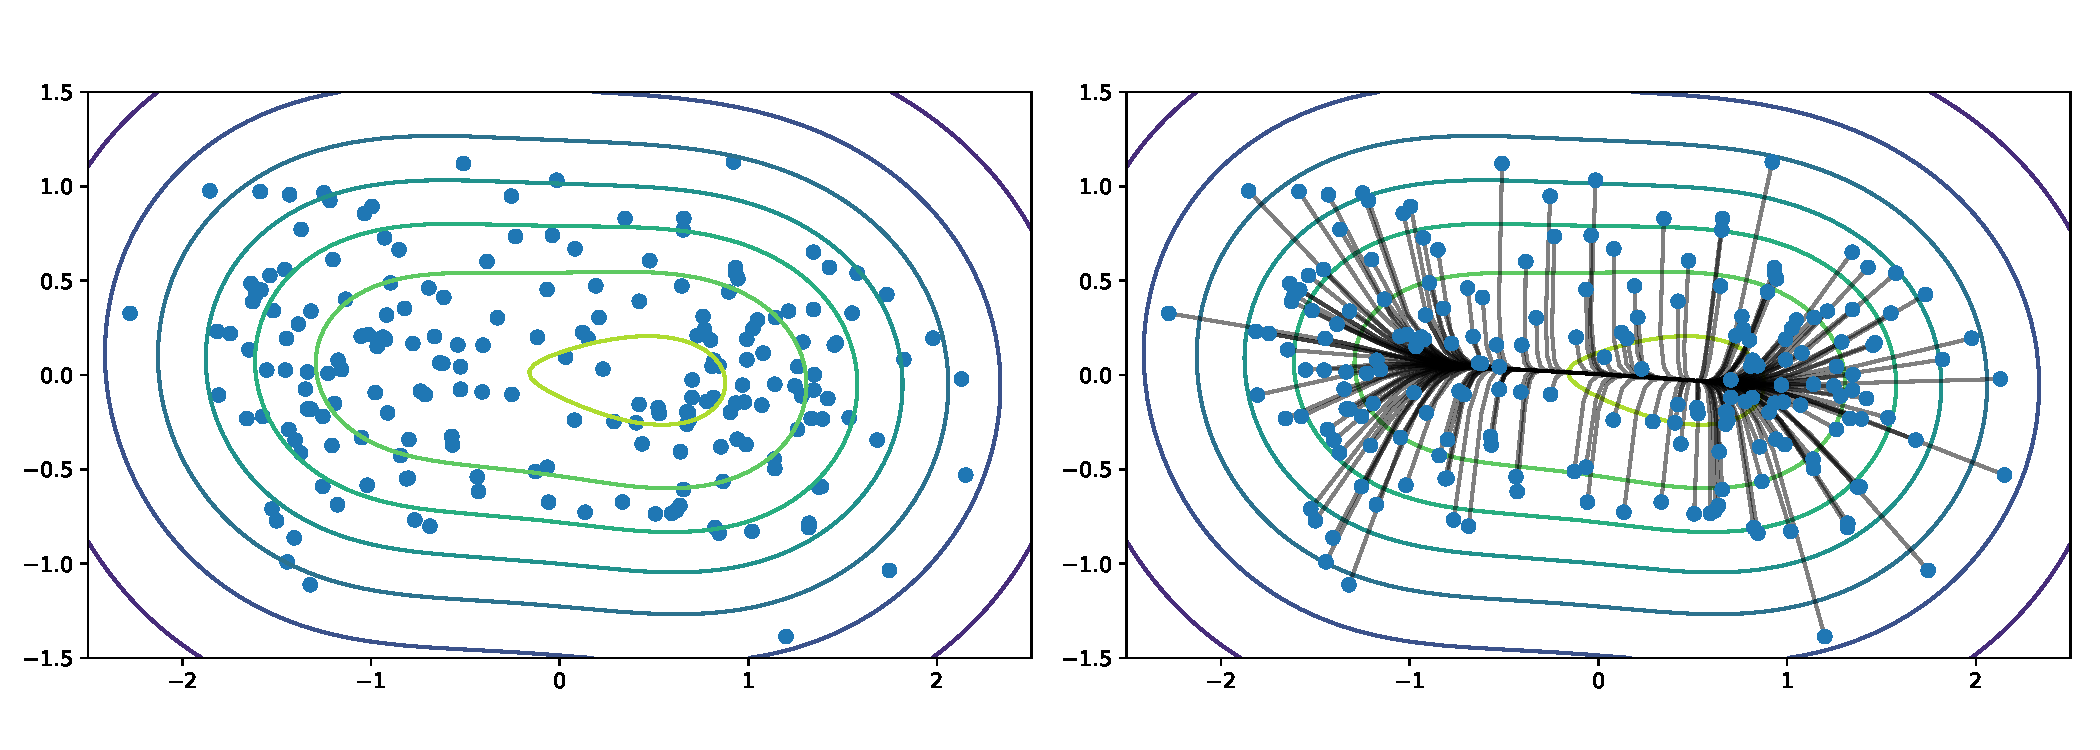
\includegraphics[height=0.4\textheight]{{{figures/contour/kde-and-trajectories-h=0.8-K=gaussian}}} \\[-2mm]
		$h=0.8$, gaussian kernel \\
		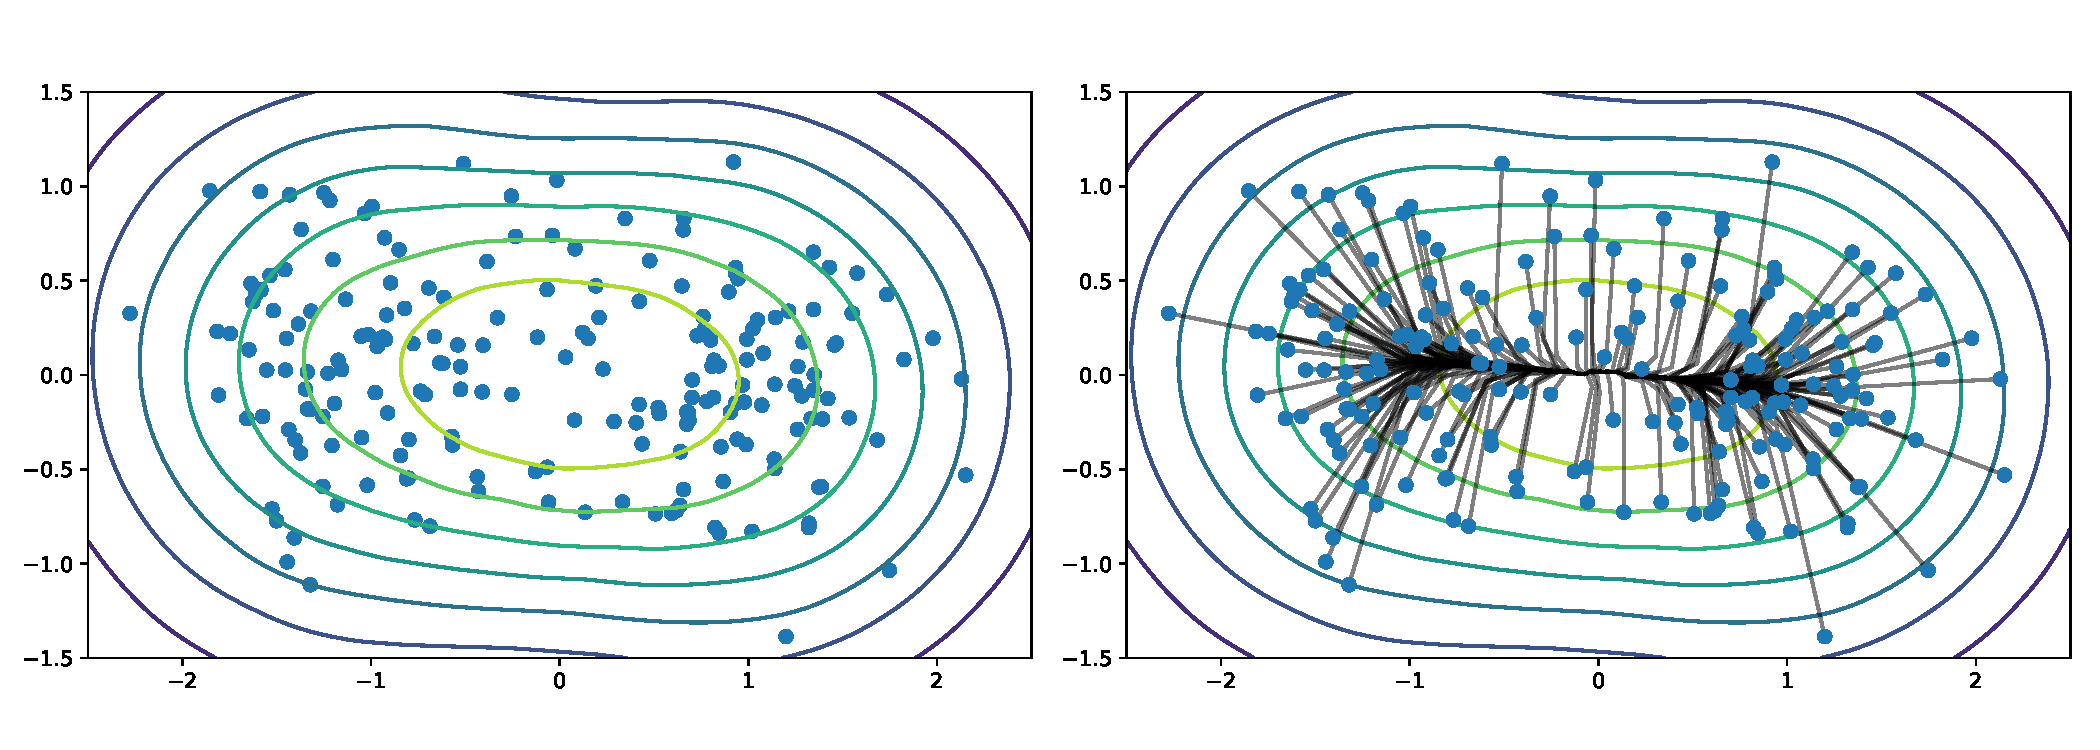
\includegraphics[height=0.4\textheight]{{{figures/contour/kde-and-trajectories-h=1.7-K=uniform}}} \\[-2mm]
		$h=1.7$, uniform kernel
	\end{tabular}
\end{figure}
\end{frame}


\subsection{Speedup methods and discussion}

\begin{frame}{Speedup methods}
	The mean shift algorithm has computational complexity $\mathcal{O}(Tn^2)$, with $T$ being the number of iterations until convergence.
	
	\begin{itemize}
		\item \textbf{Parallelization} of iteration procedure. The trajectories are computational independent.
		
		\item \textbf{Sampling} of the dataset. Only perform it on a subset.
		
		\item \textbf{Bucketing} the dataset. Reduce number of possible positions.
		
		\item Use of \textbf{spatial data structures}. For kernels with compact support only the data points in the neighborhood are relevant.
		
		\item \textbf{Merging} of trajectories. When two trajectories get close to each other it is likely that they converge to the same point.
	\end{itemize}
\end{frame}


\begin{frame}{Discussion}
\textbf{Advantages}
\begin{itemize}
	\item No prior assumption on cluster shapes. Complex and non-convex shapes are possible.
	\item Only has one tuning parameter, the bandwidth.
	\item No restriction on number of clusters.
	%\item Cluster centroids are local maxima of the density.
	\item Outliers do not affect the clustering.
\end{itemize}
\textbf{Disadvantages}
\begin{itemize}
	\item Density estimation fails for high dimensions ($\approx d$ > 5).
	\item Bad computational complexity $\mathcal{O}(Tn^2)$.
	\item Finding a good bandwidth is hard.
\end{itemize}
\end{frame}


\section{Application}

\begin{frame}{Application}
	\begin{itemize}
		\item Introduced by \cite{Fukunaga.1975}, but popularized for computer vision tasks \cite{Comaniciu.2002} and \cite{Comaniciu.2003}.
	\end{itemize}

\begin{itemize}
	\item Generic clustering algorithm.
	\item Image segmentation, image filtering and object tracking.
\end{itemize}
\end{frame}


\subsection{Image segmentation}

\begin{frame}{Application -- Image segmentation}
\begin{figure}	
	\begin{tabular}{cc}
		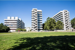
\includegraphics[height=0.4\textheight]{{{figures/kit-demo/image-resized}}} &
		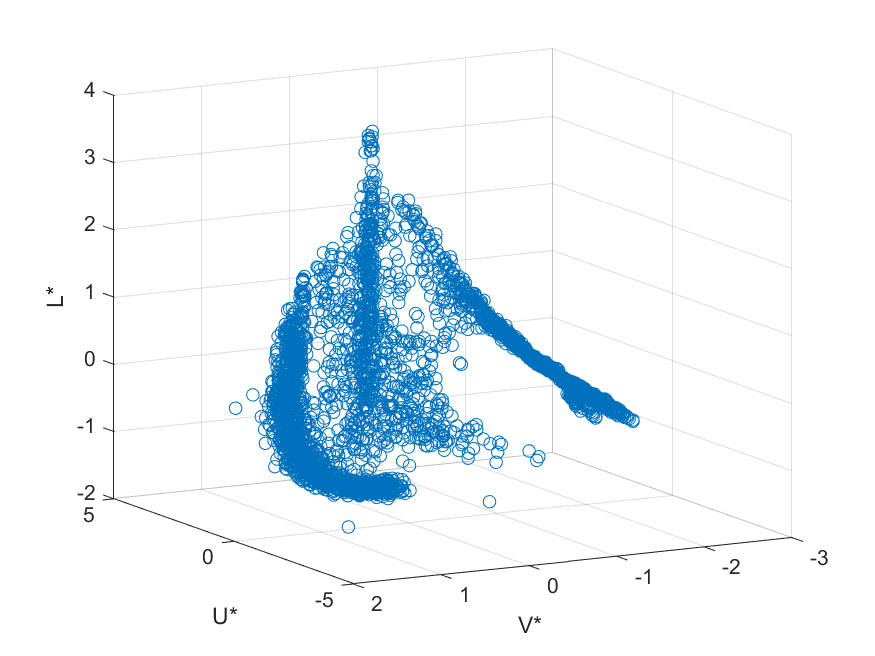
\includegraphics[height=0.5\textheight]{{{figures/kit-demo/scatter-plot}}}
	\end{tabular}
\end{figure}
\begin{itemize}
	\item Image data can be represented as data points. The pixels can be clustered and the clustering results in a segmentation of the original image.
\end{itemize}
\end{frame}

\begin{frame}{Preprocessing}
	\begin{itemize}
		\item \textbf{Image rescaling} for quicker convergence.
		\item \textbf{Color space transformation}. The CIE 1976 L*,u*,v* color space is built to approximate a perceptually uniform color space.
		\item \textbf{Feature standardization} with mean and standard deviation.
		\item \textbf{Adding spatial features}. Adding $(x, y)$ pixel coordinates to pixel data.
	\end{itemize}
\end{frame}


\begin{frame}{Image segmentation -- Gaussian kernel}
\tiny
\begin{figure}
	\begin{tabular}{cc}
		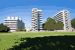
\includegraphics[height=0.3\textheight]{{figures/kit-demo/image-segmentation-h=0.1-K=gaussian}.png} &   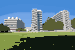
\includegraphics[height=0.3\textheight]{{figures/kit-demo/image-segmentation-h=0.2-K=gaussian}.png} \\
		(a) $h = 0.1$ & (b) $h = 0.2$ \\[6pt]
		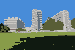
\includegraphics[height=0.3\textheight]{{figures/kit-demo/image-segmentation-h=0.3-K=gaussian}.png} &   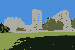
\includegraphics[height=0.3\textheight]{{figures/kit-demo/image-segmentation-h=0.4-K=gaussian}.png} \\
		(c) $h = 0.3$ & (d) $h = 0.4$ \\[6pt]
	\end{tabular}
\end{figure}
\end{frame}


\begin{frame}{Image segmentation -- Gaussian kernel}
\tiny
\begin{figure}
\begin{tabular}{cc}
	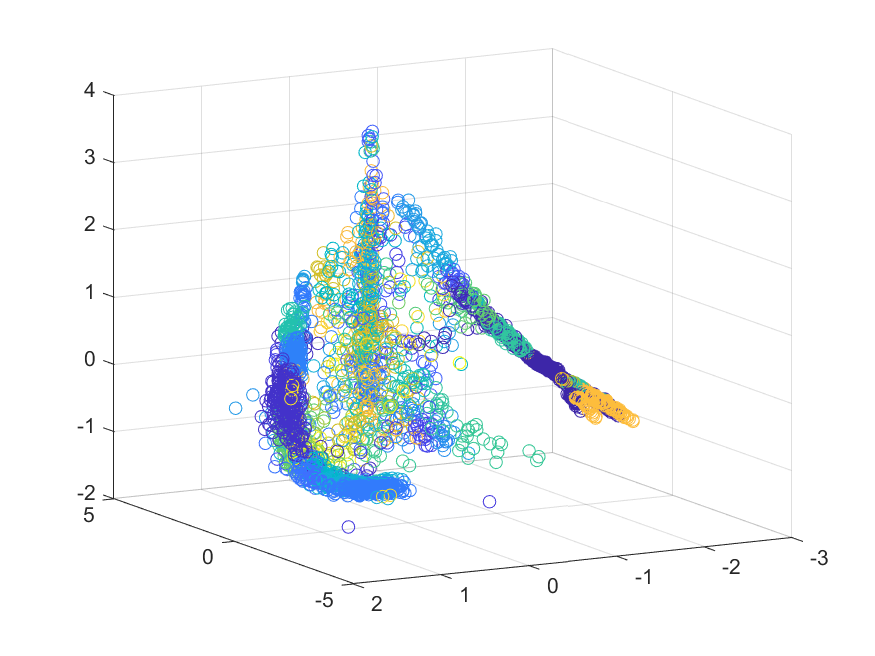
\includegraphics[height=0.3\textheight]{{figures/kit-demo/scatter-plot-h=0.1-K=gaussian}.png} &   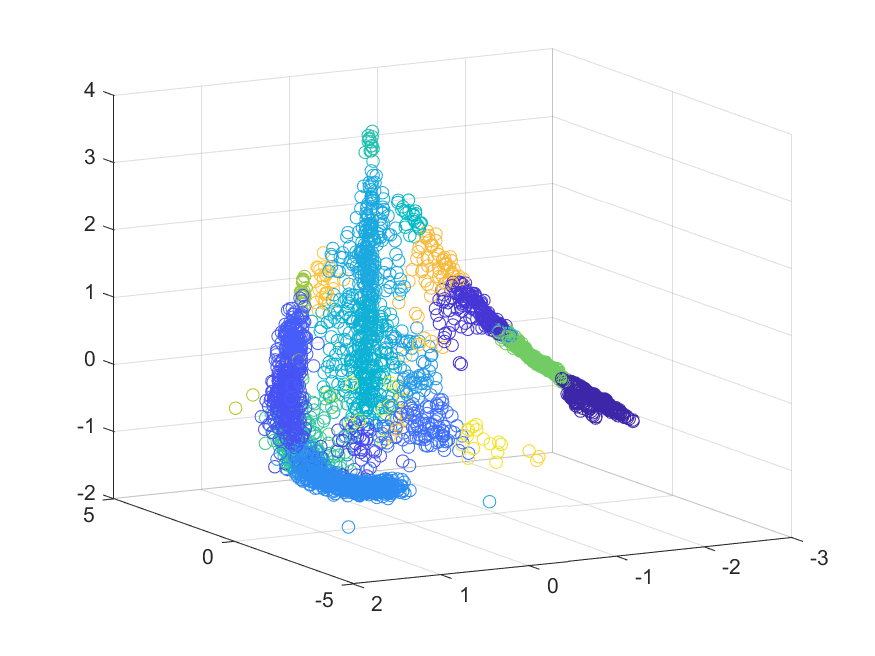
\includegraphics[height=0.3\textheight]{{figures/kit-demo/scatter-plot-h=0.2-K=gaussian}.png} \\
	(a) $h = 0.1$ & (b) $h = 0.2$ \\[6pt]
	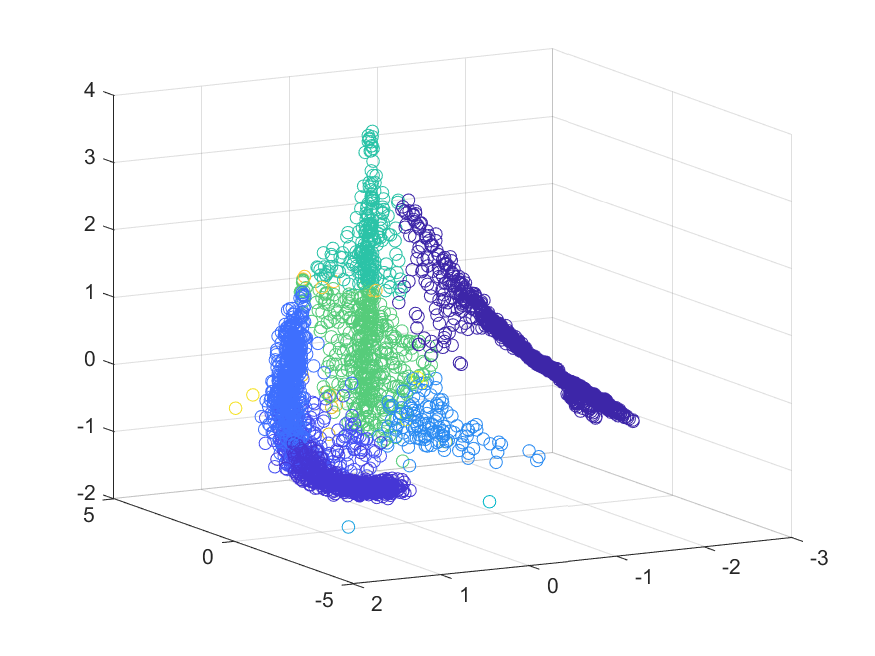
\includegraphics[height=0.3\textheight]{{figures/kit-demo/scatter-plot-h=0.3-K=gaussian}.png} &   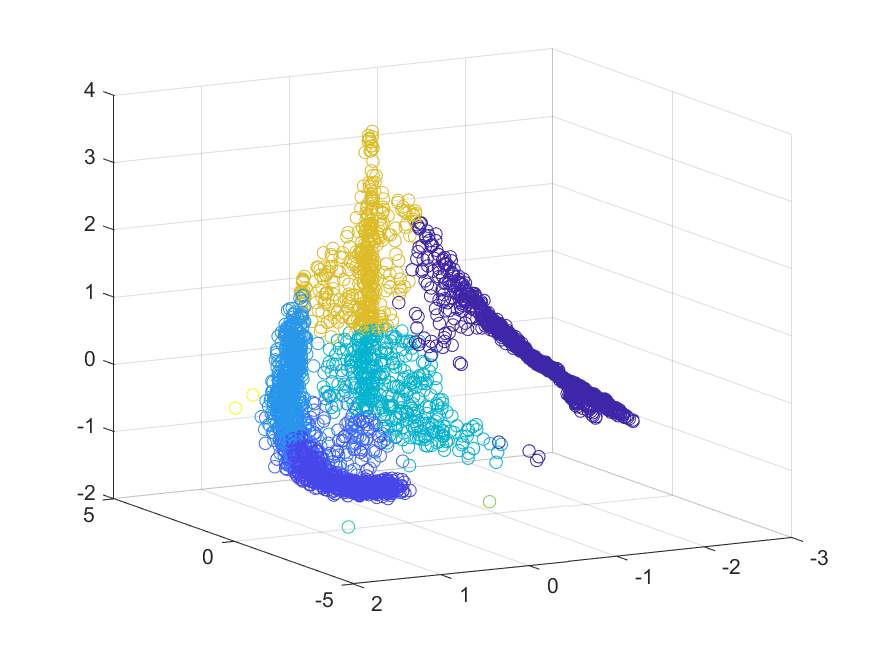
\includegraphics[height=0.3\textheight]{{figures/kit-demo/scatter-plot-h=0.4-K=gaussian}.png} \\
	(c) $h = 0.3$ & (d) $h = 0.4$ \\[6pt]
\end{tabular}
\end{figure}
\end{frame}


\begin{frame}{Image segmentation -- Uniform kernel}
\tiny
\begin{figure}
\begin{tabular}{cc}
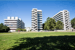
\includegraphics[height=0.3\textheight]{{figures/kit-demo/image-segmentation-h=0.1-K=uniform}.png} &   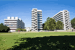
\includegraphics[height=0.3\textheight]{{figures/kit-demo/image-segmentation-h=0.2-K=uniform}.png} \\
(a) $h = 0.1$ & (b) $h = 0.2$ \\[6pt]
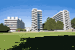
\includegraphics[height=0.3\textheight]{{figures/kit-demo/image-segmentation-h=0.3-K=uniform}.png} &   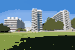
\includegraphics[height=0.3\textheight]{{figures/kit-demo/image-segmentation-h=0.4-K=uniform}.png} \\
(c) $h = 0.3$ & (d) $h = 0.4$ \\[6pt]
\end{tabular}
\end{figure}
\end{frame}


\begin{frame}{Image segmentation -- Uniform kernel}
\tiny
\begin{figure}
\begin{tabular}{cc}
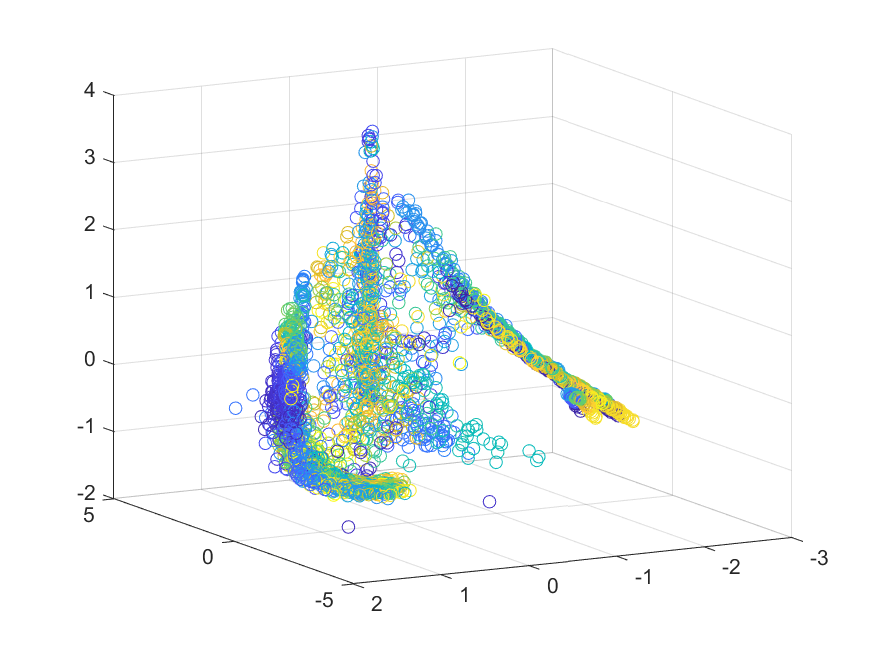
\includegraphics[height=0.3\textheight]{{figures/kit-demo/scatter-plot-h=0.1-K=uniform}.png} &   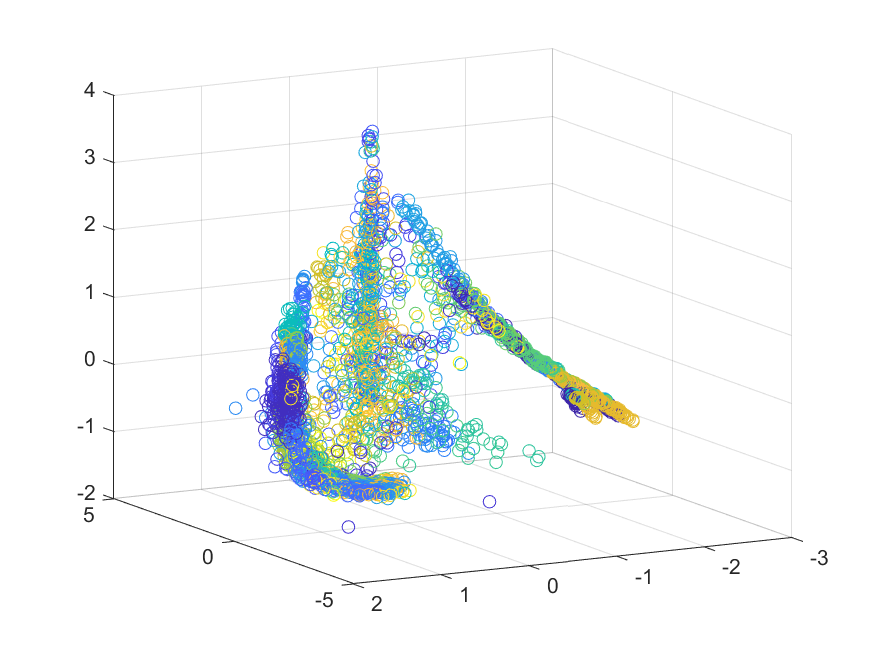
\includegraphics[height=0.3\textheight]{{figures/kit-demo/scatter-plot-h=0.2-K=uniform}.png} \\
(a) $h = 0.1$ & (b) $h = 0.2$ \\[6pt]
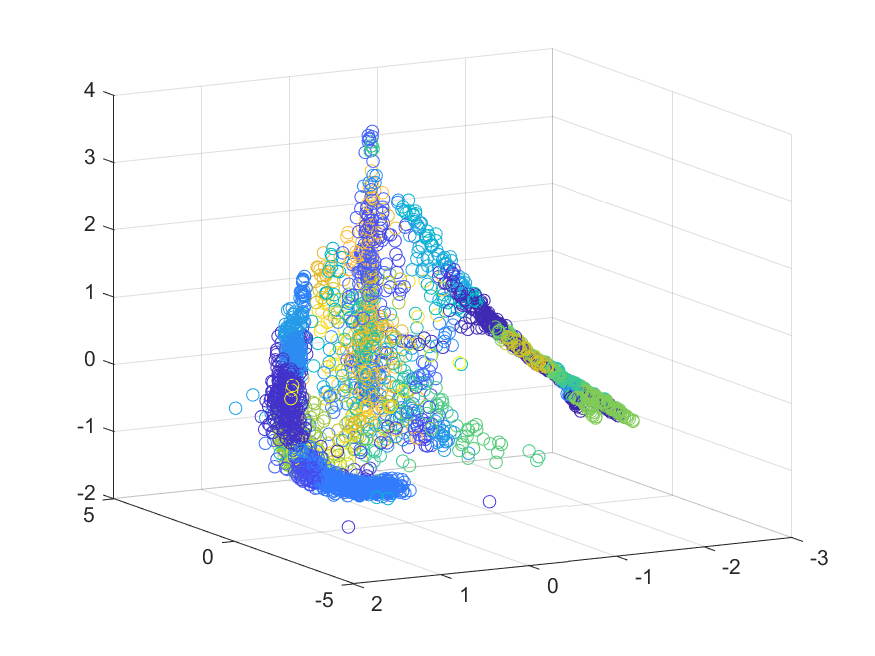
\includegraphics[height=0.3\textheight]{{figures/kit-demo/scatter-plot-h=0.3-K=uniform}.png} &   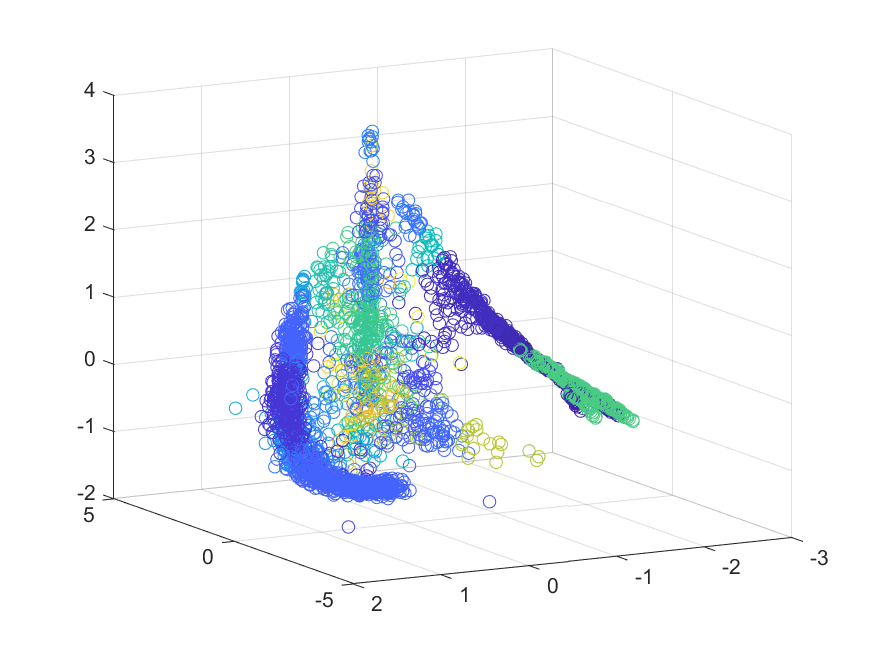
\includegraphics[height=0.3\textheight]{{figures/kit-demo/scatter-plot-h=0.4-K=uniform}.png} \\
(c) $h = 0.3$ & (d) $h = 0.4$ \\[6pt]
\end{tabular}
\end{figure}
\end{frame}


\begin{frame}{Results}
	\centering
	\includegraphics<1>[height=0.4\textheight]{figures/segmentation/segmentation-results-100_0109}
	\includegraphics<1>[height=0.4\textheight]{figures/segmentation/segmentation-results-palovigna}
	\includegraphics<2>[height=0.4\textheight]{figures/segmentation/segmentation-results-culzeancastle}
	\includegraphics<2>[height=0.4\textheight]{figures/segmentation/segmentation-results-ireland_62_bg_061502}
	\includegraphics<3>[height=0.4\textheight]{figures/segmentation/segmentation-results-dscf3583}
	\includegraphics<3>[height=0.4\textheight]{figures/segmentation/segmentation-results-pic109250805856}
\end{frame}


\begin{frame}{Limitations}
\centering
\includegraphics<1>[height=0.4\textheight]{figures/segmentation-bad-results/segmentation-results-b19objects118}
\includegraphics<1>[height=0.4\textheight]{figures/segmentation-bad-results/segmentation-results-bbmf_lancaster_july_06}
\includegraphics<2>[height=0.4\textheight]{figures/segmentation-bad-results/segmentation-results-dsc_0959}
\includegraphics<2>[height=0.4\textheight]{figures/segmentation-bad-results/segmentation-results-dscn2154}
\end{frame}


\appendix

\begin{frame}[allowframebreaks]{References}
	%\printbibliography
	
	\bibliographystyle{agsm}
	\bibliography{../latex/KDEaMSC}
\end{frame}

\begin{frame}{Figures}
	\begin{itemize}
		\item ``KIT chemical faculty building'' picture. Copyright by KIT.
		\item Segmentation pictures. ``segmentation evaluation database'' from \cite{Alpert.2012}.
		\item All other illustrations were done by the author.
	\end{itemize}
\end{frame}

\beginbackup

\backupend

\end{document}
